\part{Planning prévisionnel}

\section{Étapes du projet}
 
Notre projet comporte 4 étapes principales. Chacune de ces étapes aura une date de remise définie dès le début du projet. 

\paragraph{La rédaction du cahier des charges}

Dans cette étape, nous avons principalement eu besoin de rédiger la demande du client. 
Nous avons aussi eu à étudier le fonctionnement du logiciel Royal que l'on a choisi d'ameliorer afin d'arriver au but visé.
Les contraintes liées à l'amélioration de ce logiciel nous permettent de definire la faisabilité des differentes fonctions. 

\paragraph{La rédaction du dossier d'analyse}

Dans cette partie, nous aurons à approfondir l'analyse ainsi que la conception des différentes fonctions et le fonctionnement du logiciel Royal. 
Nous définirons aussi les différents outils utilisés afin de développer le projet, tel qu' 
Eclipse \footnote{Site de l'IDE Eclipse : http://www.eclipse.org/} 
pour le développement JAVA, ou encore 
PowerAMC \footnote{Site officiel de PowerAMC : http://www.sybase.fr/products/modelingdevelopment/poweramc}
pour la réalisation des MCD.

\paragraph{La réalisation d'un premier prototype}

Afin de rendre un prototype, le 5 Décembre 2011, répondant aux principales demandes de l'utilisateur nous développerons les fonctions de priorités 1 et 2.
Pour permettre l'implémentation de certaines de ces fonctions, nous aurons à modifier la base de données en suivant le modèle modifié dans l'étape précédente.  

\paragraph{La finalisation du projet}

Cette étape sera la dernière de notre projet et devra être effectuée avant le 19 Janvier 2012 (date de livraison de notre projet).
Pour la finalisation, nous développerons les fonctions de priorités inférieures afin de répondre aux besoins moins importants. 

\section{Estimation du temps nécessaire}
Pour la réalisation des estimations de temps nécessaire à la réussite de ce projet,
nous nous sommes basés sur deux méthodes. 

La première méthode choisie est l'\emph{estimation par analogie}.
Elle correspond à réaliser une proportion entre les différentes étapes du projet. 

\begin{tabular}{|l l|l|l|}
\hline
&& Durée proportionnelle & Durée concrète \\
\hline
Opportunité & Étude préalable & 10\% & 60h \\
\hline
Élaboration & Conception de la solution détaillée & 30\% & 180h \\
\hline
Construction & Développement & 50\% & 300h \\
\hline
Transition & Mise en œuvre & 10\% & 60h \\
\hline
\end{tabular}

Avec cette méthode, nous avons une estimation de travail de $60 + 180 + 300 + 60 = 600$ heures. 

\section{Planification des délais}

Pour la planification des délais, nous avons utilisé la méthode du \emph{diagramme de GANTT}.
\begin{figure}[h]
\begin{center}
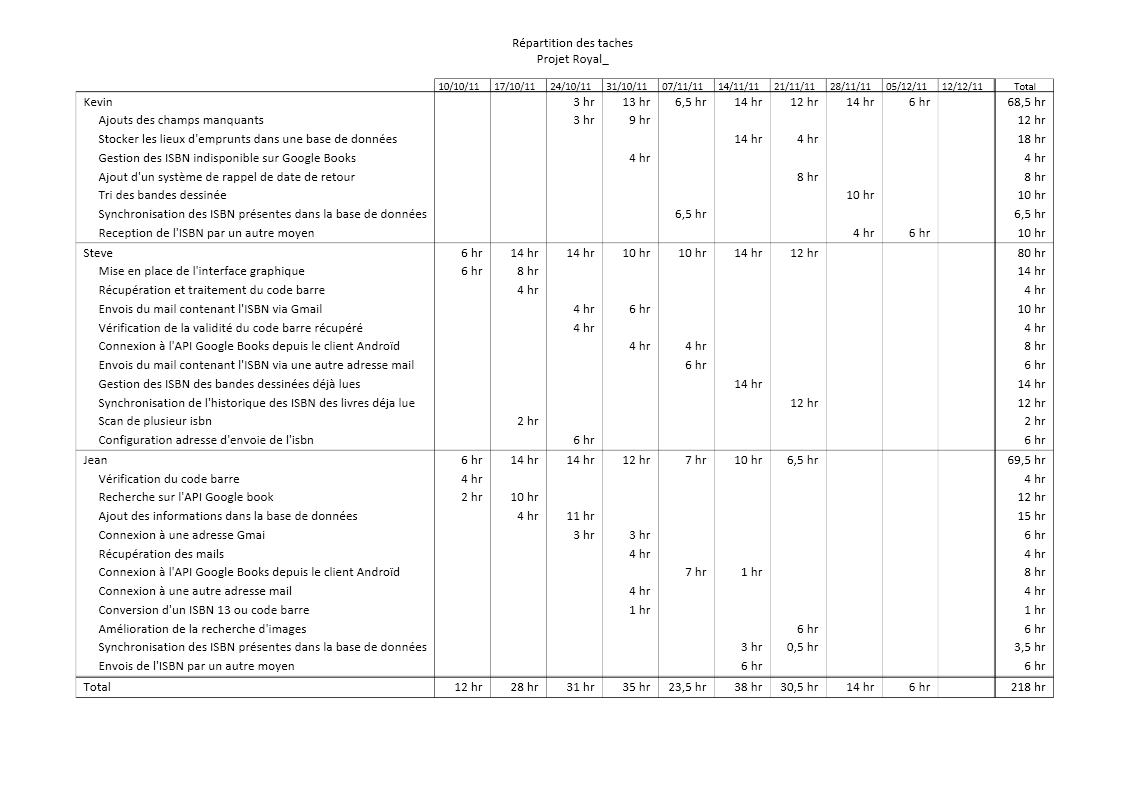
\includegraphics[height=12cm]{../repartition_des_taches.png}
\end{center}
\caption{Éstimation de notre temps de travail}
\end{figure}
\subsection{Diagramme de GANTT}

Pour la planification du projet par fonctions, nous avons utilisé un \emph{diagramme de GANTT} qui correspond à peu près à la méthode \emph{analytique} (excepter qu'elle ne prend en compte que les phases de conception).
\begin{wrapfigure}[40]{l}{15cm}
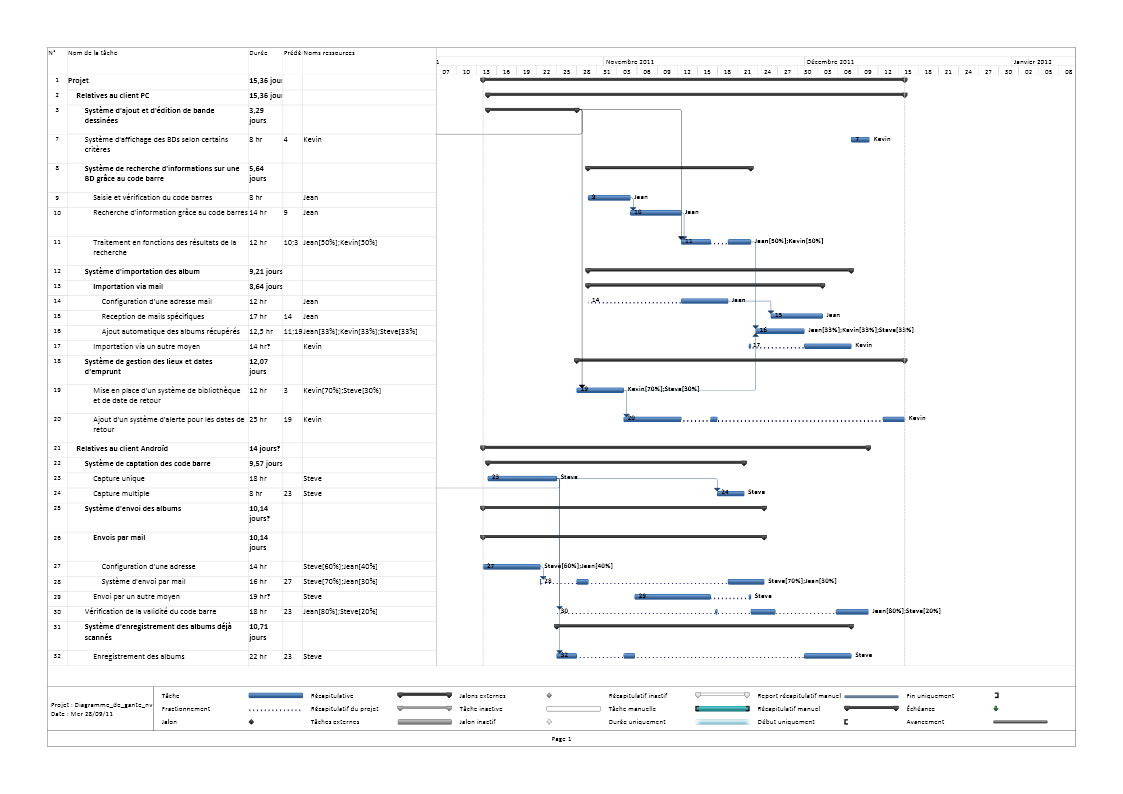
\includegraphics[width=15cm]{../Diagramme_gante.png}
\end{wrapfigure}
\clearpage

\subsection{Comparaison des méthodes}
\emph{Microsoft Project} a caculé un temps de développement de \textbf{253h}. 
Avec notre estimation par analogie, nous avons trouvé un temps consacré au développement de \textbf{300h}. 
Nous pouvons donc dire que globalement, les résultats concordent. 
Ceux-ci peuvent donc être fiables, et le temps réel devrait se situer entre 253 et 300h de codage. 

\subsection{Difficultés encourues} 
L'estimation du temps de réalisation des fonctionnalités à été un problème. 
En effet, le manque d'expérience dans le domaine du travail en équipe nous empêche de bien définir si nos enchainements entre la réalisation des fonctionnalités se dérouleront bien comme prévu, et si nous arriverons à travailler ensemble efficacement. 

Le deuxième problème dans l'estimation vient de notre manque d'expérience en tant que programmeur :
L'instabilité des connaissances acquises nous fera peut-être perdre du temps dans l'apprentissage de quelque chose qu'on aura estimé plus simple à assimiler. 
